
\chapter{A modular synthesis engine}

\epigraph{We can now see that the whole becomes not merely more, but
  very different from the sum of its parts.}{\emph{More is Different:
  Broken Symmetry and the Nature of the Hierarchical Structure of
  Science}\\\textsc{Philip Warren Anderson}}

\section{Analysis}

In the previous chapter we built a system for sound representation,
processing, and interfacing. In such system, interactions
between different processing elements is hard-coded in the control
flow of the program itself and the relations among the statically
parametrised types that intervene.

As described by requirements \ref{req:iter2-begin} to
\ref{req:iter2-end}, we shall develop a system where the basic DSP
units can be composed orthogonally and hierarchically to build complex
devices \emph{at runtime}. With the applications built on top of our
framework being targeted at live performances, it should be
particularly dynamic.

\subsection{An abstract model of a modular synthesiser}

In a modular synthesiser, the sound generation is made by
interconnecting basic processing units. Each of them might generate
sound, filter it, and can have a varying number of inputs and outputs
of different kinds. Because a module can apply virtually any
mathematical function to its inputs; we can realise any synthesis
technique --- i.e. additive, subtractive, FM/PM --- by just wiring the
available modules in an appropriate way.

We can characterise such a system by abstracting the parts of one of
these processing units. A hardware modular synthesiser can be used to
illustrate the concepts behind this, as shown by the \emph{frequency
  shifter}\footnote{A frequency shifter is a module that produces
  oscillating modifications on the frequency components of a given
  input signals, producing interesting Doppler effects, binaural
  effects, vibratos, and so on.} in figure \ref{fig:hwmod}. We can thus
taxonomise its parts as in the following; we will later use this
terminology in our design.

\begin{description}
\item[Input ports] These are the signals that come from another module. In
  the example figure we can see a \emph{input} signal that carries an
  arbitrary sound wave to be frequency-shifted, and a \emph{CV in},
  which is used to modulate the shift parameter. In a hardware module
  we can consider as an input anything that can go through a wire,
  thus we are no limited just to analog time-domain signals, but we
  can consider a digital MIDI input of a synthesiser as an input
  signal too.

  In our software system we are even less constrained, and our system
  should cope with signals of any kind --- i.e. of any type, in the
  programming language sense. Note also that an input might remain
  disconnected during execution of the synthesis graph, and a proper
  default behaviour should be implemented in that case.

\item[Output ports] These are the signals that the module sends to other
  modules. They are of the same nature than their input counterparts.

  In order to connect an output to an input, the kind of signals that
  flows through them must match; in a computer based digital system
  this should be checked and proper error handling must come into
  action if necessary or maybe some automatic conversion mechanism if
  safe and applicable.

  Note that while on and hardware synth inputs and outputs are
  generally related in a one-to-one manner --- unless we do not
  consider a hub/split or a mixer a module by itself but a connection
  device --- in software we can relate them in a one-to-many fashion,
  as the value produced in an \emph{output port} can be read several
  times by different modules if it has its own memory.

\item[Parameter controls] These allow the user to tune the different
  settings of the device. In a hardware device, they are most of the
  time represented by a knob or a slider, but modern synthesisers
  include bidimensional touchpads and other input devices for
  controlling the process.

  Note that, at this stage, the notion of a \emph{parameter} or
  \emph{control} is not directly related to how it might be
  represented to the user --- like a text-box, virtual knob, or
  whatosever --- but to the abstractions that the a DSP module uses to
  get input from outside of its inner processing function. Just like
  an input port, it should be of any type. For example, any control
  that is naturally representable with a knob or slide is quite often
  a \emph{float} parameter.

  The reader might wonder how is this different from an input port in
  a software system. On the one hand, controls do not have any
  built-in interconnection system. On the other hand, the
  synchronisation mechanisms used to pass the values through controls
  and ports are quite different. This is so because while the
  information that goes through ports is to be used only by the DSP
  modules, controls get input from the user interface thread, thus
  requiring special care. We will discuss this further in the next
  section.

\item[Status controls] These provide feedback to the user about
  relevant parts of the state of the processing. In the example
  figure, a red led is light up when the output signal exceeds the
  \emph{clipping value} --- i.e. the upper threshold of the admissible
  range of the amplitude of the signal --- suggesting the user to
  lower the gain to avoid annoying distortion. Everything that have
  been said about parameter control applies here. Once again, what is
  important is the abstraction not the visual representation; those
  the aforementioned example would be a \emph{boolean} status control in our
  system, that might be represented by any other means.
\end{description}

\begin{figure}
  \centering
  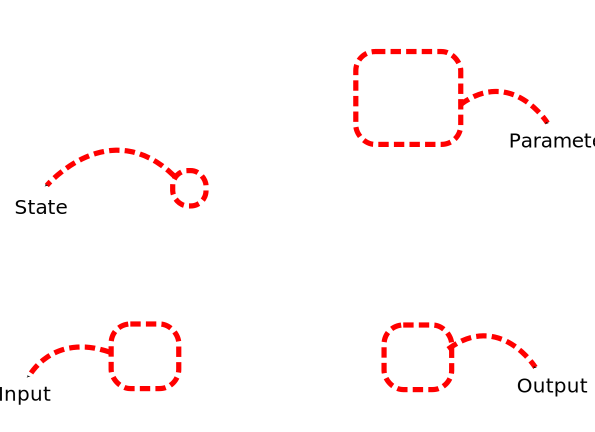
\includegraphics[width=.9\textwidth]{pic/hwmod.png}
  \caption{Components of a synthesis module illustrated in a standard
    \emph{frequency shifter}.}
  \label{fig:hwmod}
\end{figure}

A collection of modules and the connections among them is called a
\emph{patch}. In a hardware modular synthesiser, these are assembled
in special racks that have slots satisfying some standard to place the
modules in them --- for example, the module in the figure fits in
\emph{eurorack} slots. In many software synths, and specifically in
the one we are developing, patches can be arranged hierarchically. We
can visualise this as if we could put a whole rack into a black box
with holes to expose certain controls and ports to the outside, and
then place this box in a larger rack. This is very useful in a
software synthesiser; for example, one could build a complex patch out
of low-level processing primitives and expose a simplified
interface. Some software, like Reaktor, call these patches
\emph{instruments}. This arrangement can then be stored into a file
for later use. On the Internet one can find many collections of these
ready-to-use patches, and there are even commercial packages developed
by professional sound designers.

The \emph{conceptual class diagram} in figure \ref{fig:graphconcept}
summarises all this. Note that this is a conceptual class diagram, not
a design one, so there is not necessarily a direct match to the
classes in the actual code, not even terminologically.

\begin{figure}[h]
  \centering
  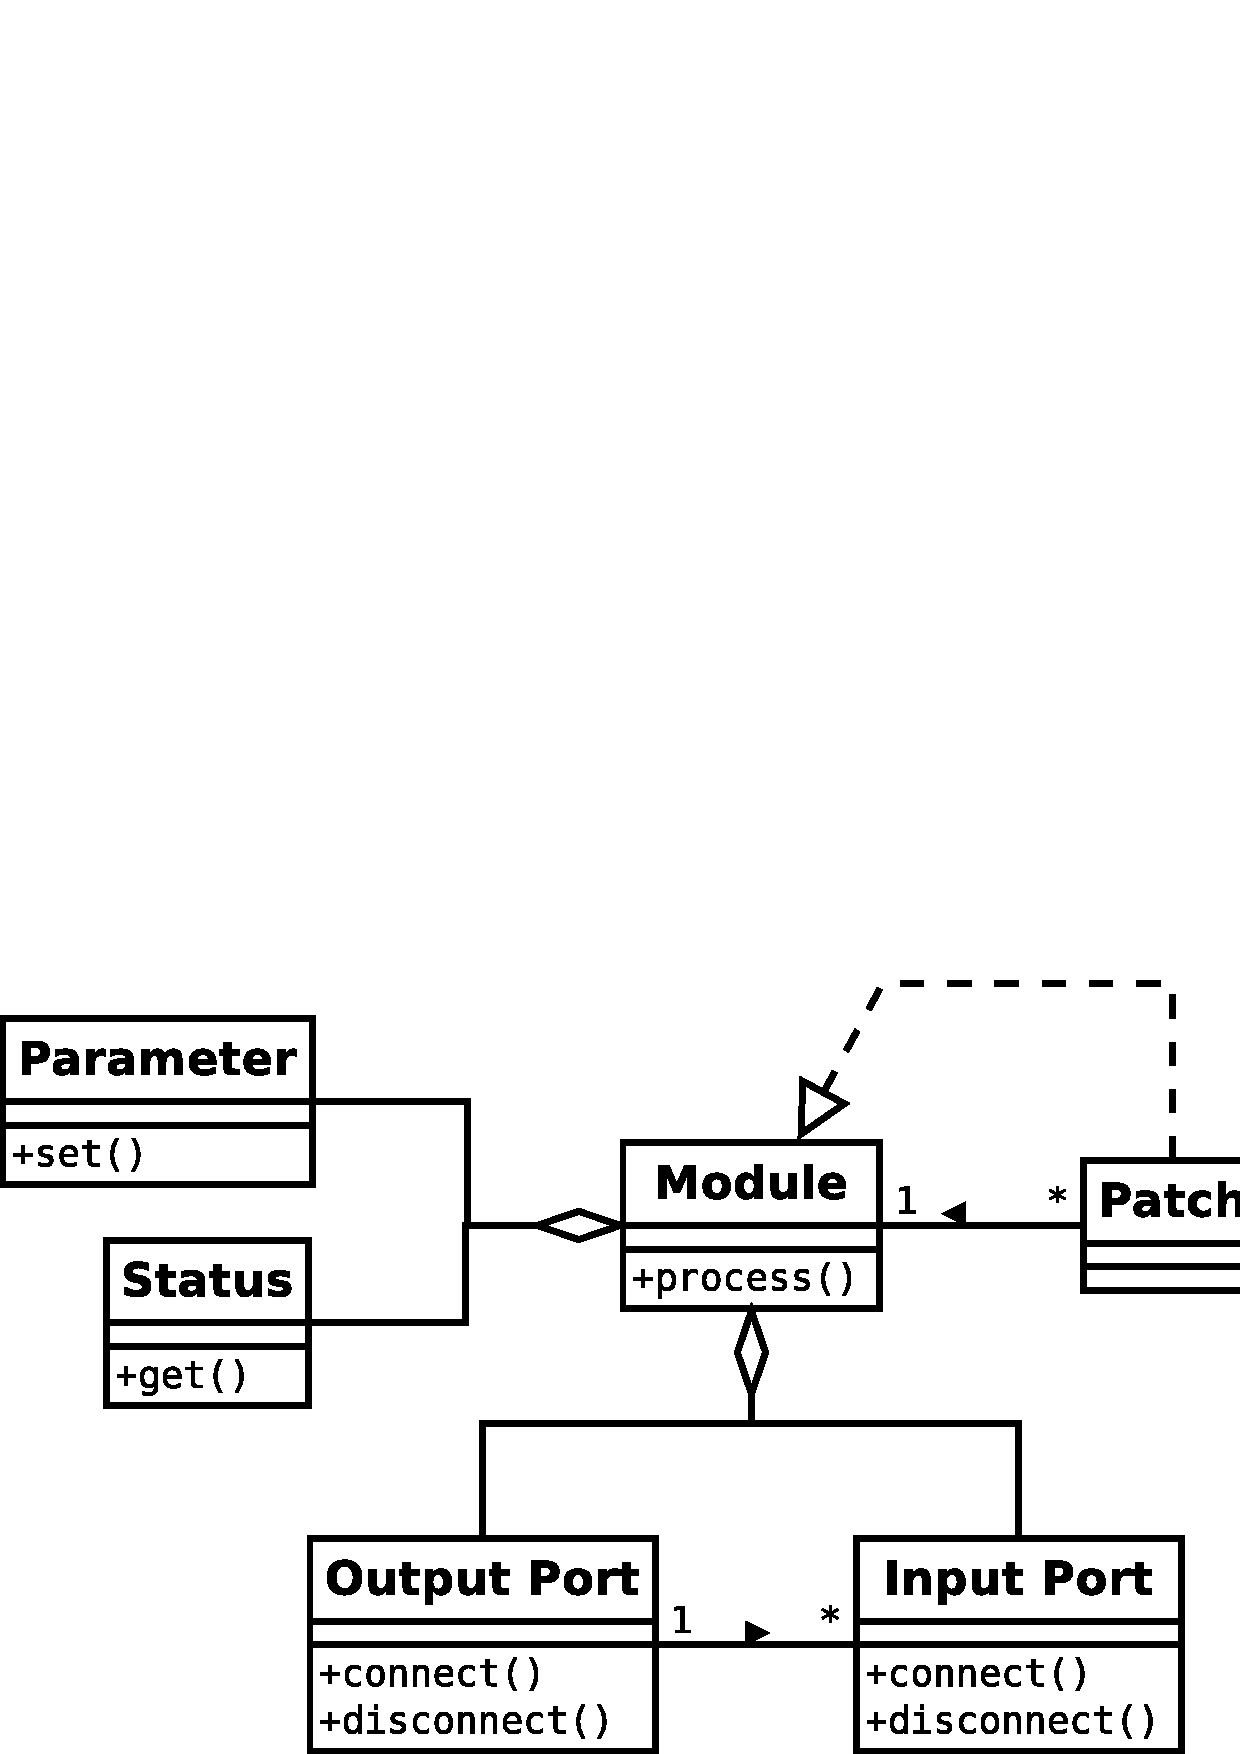
\includegraphics[width=.9\textwidth]{pic/graph-concept.pdf}
  \caption{Conceptual class diagram of the modular synthesis main entities.}
  \label{fig:graphconcept}
\end{figure}

\subsection{Software real time synthesis concerns}
\label{sec:rtsynth}

Our system generates the audio in real-time sending it directly to an
output device --- a sound-card. Even more, it is specially targeted at
live performances, so every operation should be designed such that it
does not disrupt the audio generation process and generates no kind of
noise. For example, in some software modular synths changing a
connection among ports triggers a recomputation of the dependencies
among modules to generate a compiled form of the patch for easier
execution; but that often that takes long enough to produce a small
buffer underrun --- i.e. an audible click --- as it might involve
doing non-linear computations or locking certain mutexes to
synchronise the state with the user thread. Actually, the port
reconnection issue requires special care, as we will discuss in
section \ref{sec:modports}. Because of \emph{dynamic-patching} we
should expect the topology of the synthesis graph to change a lot
during a live performance.

To better understand this problem we should understand how audio is
usually processed in real-time, thus feeding us with proper
terminology and knowledge to later tackle the issue. While this might
seem like a design issue to some, this is such a universal structure
that it shall be consider as a fixed constraint to be analysed than a
design decision itself.

Ideally, we would produce each sample one at a time and send it to the
output device. However, because we have to produce, at least, 44100
samples per second --- more in some professional applications ---
traversing all the synthesis system for every frame involves many
function calls, some of them even require dynamic dispatch in an
extensible system like ours, leading to a too low performance to
deliver the samples on time. For this reason, audio is processed
blocks of \emph{block size} samples in tight loops. This \emph{block
  size} might match the device's buffer size or it might be
smaller. Parameter and status values are updated only in between
blocks. Thus, we should try to keep the block size as low as possible
to avoid noticeable latency, and most professional audio software
allow changing this parameter to fit the machine processing power. A
sensible block size is 64 samples, like Pure Data's default. Using the
terminology in \cite{boulanger10audio}, we can distinguish between
\emph{audio rate} --- i.e. the frame rate as described in the previous
chapter --- and \emph{control rate}, which is the sampling frequency
of control signals --- i.e. the signals that produce only one sample
per processing block:

\begin{equation}
  control\mbox{-}rate = \frac{audio\mbox{-}rate}{block\mbox{-}size}  
\end{equation}

Note that control signals are not restricted to what we labelled as
\emph{controls} in the previous sections. In fact, through a
\emph{port} may flow signals at audio rate if their signal type is
that of an audio buffer that holds a block of samples, or at control
rate if their signal type is that of a single sample, like a
\type{float} or \type{double}.

Interleaving the audio computation within the user-interface loop is
not plausible; thus the audio processing lives in its own thread/s. In
fact, as we saw in the previous system, some audio output interfaces
like Jackd control the audio thread themselves invoking the processing
function through a callback. Our own device API wrapper that we
developed in the previous chapter promotes this kind of asynchronous
output. The inverse of the control rate, that we may call the
\emph{control period}, provides a very explicit deadline for block
processing function. Missing the deadline might not kill people, but
it would produce an unpleasant clicking noise and thus we have to do
as much as possible to meet the deadline\footnote{In fact, in the
  middle of a live performance with a $10^5$ watts sound system,
  consequences might be more severe as it seems superficially :)}. Our
system can be categorised as \emph{soft real-time}
\cite{tanenbaum07mos}. Apart from trying to get real-time
priority in the audio thread, we have to take special care when
developing the program, and this will deeply influence the design:

\begin{enumerate}

\item Avoid system calls in the audio thread. System calls produce a
  context switch and it can take quite long until the audio thread is
  preempted back; at least too much to meet the deadline. This is
  specially true for I/O system calls. In the previous chapter we
  already provided some devices to avoid this problem, like the
  caching file readers.

\item Avoid contending for a \emph{mutex} or some other kind of lock
  with the user thread. Without special support from the operating
  system --- like priority inheriting mutexes --- this can lead to
  priority inversion \cite{kim03basic}. Even in the later case, the
  context switch produced by the contention gives good chances to miss
  the deadline until the audio thread is preempted. The overhead of
  locking a mutex when there is no contention is negligible in most
  operating systems, and it definitely is in Linux which uses
  \emph{futexes} (Fast User-space Mutex) to implement them
  \cite{franke02futex}, so using a \emph{try-lock} operation is
  usually acceptable. The rule of thumb is to never wait on a mutex in
  the audio thread, and use lock-free data structures
  \cite{valois96lockfree} or do conditional locking instead.

\item Because the dead line depends directly on the block size $n$,
  algorithms running in the audio thread should be $O(n)$. A special
  consequence of this restriction is that allocating memory in the
  heap, at least with the default allocator --- i.e. using \type{new}
  --- is forbidden. This is so because memory allocation algorithms
  are not proportional to the size of the requested block, but instead
  depend on non-deterministic properties like the pattern of memory
  usage and use complex search algorithms to find a fitting block of
  spare memory. This restriction implies that manipulating STL
  containers is forbidden too. For some special kinds of objects, a
  custom memory allocator can do the job
  \cite{alexandrescu01modern}. Sometimes, an intrusive data structure,
  like \emph{Boost.Intrusive} STL counterparts
  \footnote{\url{http://www.boost.org/doc/libs/release/doc/html/intrusive.html}}
  are enough to avoid the allocations. In other situations, we can
  release the job of allocating memory to the user thread, use custom
  data structures or any ad-hoc solution.
\end{enumerate}



\section{Design}

\label{sec:modports}

\section{Validation}

\section{Conlusion}

%%% Local Variables: 
%%% mode: latex
%%% TeX-master: "00-main"
%%% End: 
